\subsection{Systematic uncertainties}
\label{sec:systematics}

The experimental systematic uncertainties from the input analyses are incorporated in the combination as nuisance parameters in the extended likelihood fit and are profiled.
% 
Among the decay channels, correlations are taken into account for the systematic uncertainties in the jet energy scale and resolution, and the integrated luminosity.
% 
Full descriptions of the experimental systematic uncertainties per decay channel can be found in Refs.~\cite{Sirunyan:2018kta,CMS_AN_2016-442,CMS_AN_2016-366}.
% 
\tk{Make more elaborate.}


The individual $\hgg$ and $\hzz$ analyses in Refs.~\cite{} (respectively) are extrapolated to their respective fiducial phase spaces.
% 
A fiducial phase space is a conveniently chosen phase space which avoids poorly understood regions, such has for example the very-forward (high $\eta$) region, which in turn reduces the systematic uncertainties related to the extrapolation.
% 
While fiducial phase spaces are useful in the case of a single-channel analysis, there is no clear way of combining results obtained in different fiducial phase spaces.
% 
In order to combine multiple channels, the data have to unfolded to a common phase space, which commonly is chosen to be the full phase space.
% 
The main systematic uncertainties associated with this extrapolation concern uncertainties in the detector acceptances and, if not profiled in the fit, the overall normalization of Higgs boson production modes.


% ____________________________________________________________________________
% Acceptances

The combination is performed in a common phase space, chosen to be inclusive volume.
% 
The mapping of the fiducial volumes per decay channel to the inclusive phase space comes with an uncertainty on the acceptance.
% 
The acceptance uncertainty was calculated via a procedure similar to that of the theory uncertainties described in Sec.~\ref{sec:scaleuncertainties}; $\mu_R$ and $\mu_F$ were independently varied between $0.5$, $1$ and $2$, whereas the fraction $\frac{\mu_R}{\mu_F}$ was not to be less than $0.5$ or greater than $2.0$.
% 
The acceptance uncertainty per bin is then given by the minimum and maximum variations (i.e. the envelop method).
% 
In order to assess the impact on the final result, these uncertainties were added in quadrature to the existing uncertainties of the $\pt$ combination (given in Sec.~\ref{sec:noncouplingresults}).
%
The numerical results are shown in Table~\ref{tab:accuncertainties}.
% 
On solely the systematic uncertainty, the effect of the acceptance uncertainties is expected to be non-negligible in only two bins ( [45,80) and [350,60) ); on the overall uncertainty the effect is negligible throughout.
% 
For this reason acceptance uncertainties are neglected for the final results.

\begin{table}[h!]
\footnotesize
\begin{center}
\hspace*{-1cm}
\begin{tabular}{lccccccccc}
Bins                      & [0,15) & [15,30) & [30,45) & [45,80) & [80,120) & [120,200) & [200,350) & [350,600) & [600,infinity)  \\
Acc. uncertainties        & 0.6\%   & 1.3\%    & 2.8\%    & 5.7\%    & 1.0\%     & 1.7\%      & 4.1\%      & 10.2\%     & 28.8\%  \\
Rel. change in syst. unc. & 0.3\%   & 0.7\%    & 4.1\%    & 19.7\%   & 0.3\%     & 1.8\%      & 2.0\%      & 7.6\%      & 1.0\%   \\
Rel. change in tot. unc.  & 0.0\%   & 0.1\%    & 0.3\%    & 1.2\%    & 0.0\%     & 0.1\%      & 0.2\%      & 0.3\%      & 0.2\%   \\
\end{tabular}
\end{center}
\caption{
    Acceptance uncertainties and the relative change they manifest when added in quadrature to the uncertainties of the $\pt$ combination.
    }
\label{tab:accuncertainties}
\end{table}


% ____________________________________________________________________________
% xH normalization uncertainty

For certain measurements the production cross sections of non-$\ggh$ production modes are assumed to be their respective SM value.
% 
In these cases, the uncertainty in the inclusive production cross section from non-$\ggh$ modes, determined to be about 2.1\%~\cite{deFlorian:2016spz}, has been taken into account as a nuisance parameter.
% 
\tk{Explain how obtained}


\tk{From AN:}
% 
In the cases that only the cross section from ggH is to be fitted (in the $\pt^\text{ggH}$ combination and for all the coupling fits), the contribution from other production mechanisms (from now referred to as ``xH'') needs to be subtracted.
% 
The xH production comes with an uncertainty, which surmounts to about 2.1\% inclusively, obtained by adding up in quadrature the uncertainties of all the individual production modes (numbers from Ref.~\cite{deFlorian:2016spz}).
% 
The uncertainty is assumed to flat in $\pt$, and is implemented as a nuisance parameter in the fit.
% 
The $\pt^\text{ggH}$ spectrum is shown in Fig.~\ref{fig:xH_uncertainty_impact} with and without the uncertainty on xH included.
% 
The uncertainty manifests itself visibly in the systematic uncertainty, although the combination result is not significantly altered.
% 
The xH uncertainty is applied to the $\pt^\text{ggH}$ combination and for all the coupling fits.

\begin{figure}[hbtp]
  \begin{center}
    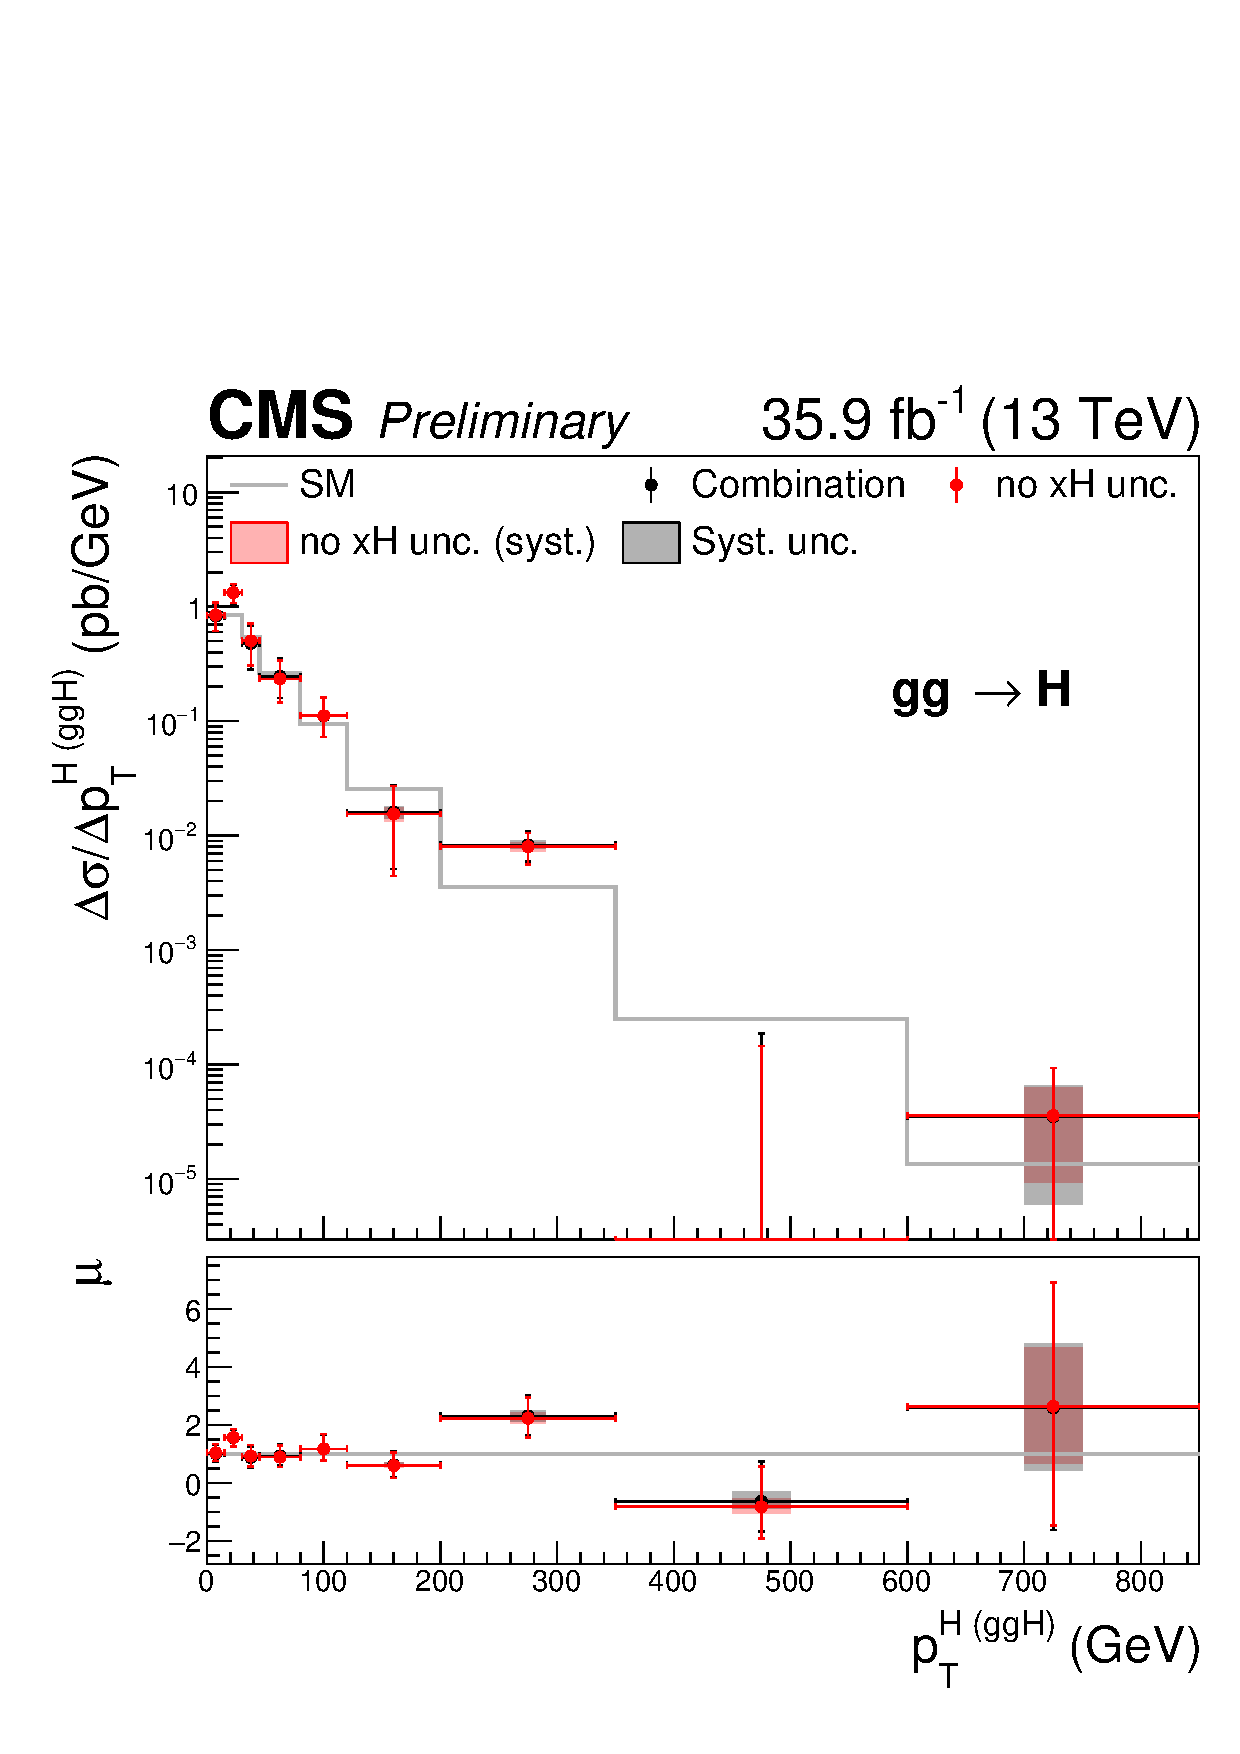
\includegraphics[width=\halflinewidth]{img/differentials/comparison_including_xH_unc.pdf}
    % 
    \caption{
        Combination of $\pt^\text{ggH}$, using the $\hgg$, $\hzz$ and $\hbb$ decay channels. 
        }
    \label{fig:xH_uncertainty_impact}
  \end{center}
\end{figure}

